\documentclass[tikz,border=4pt]{standalone}
\usetikzlibrary{positioning}

\begin{document}
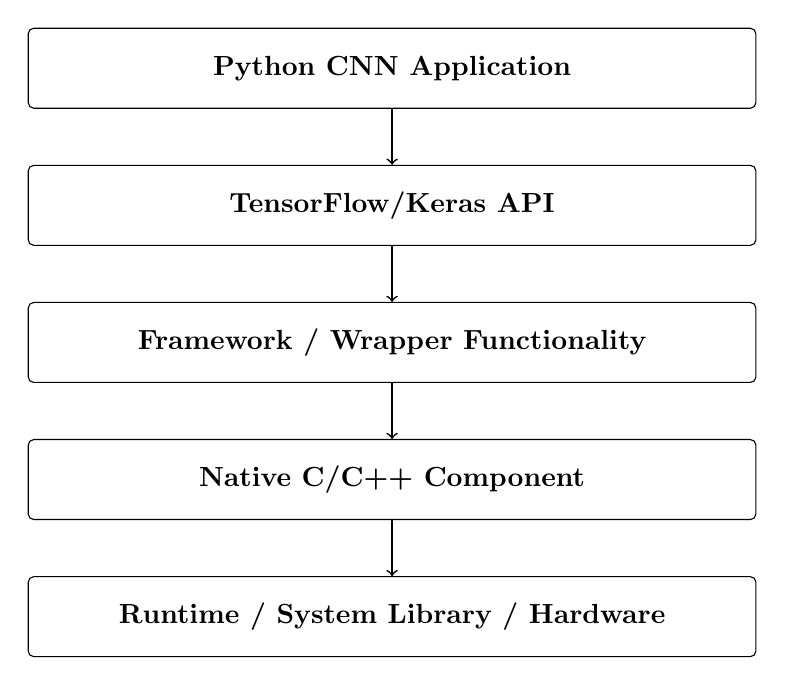
\begin{tikzpicture}[
  stage/.style={
    draw,
    rounded corners=2pt,
    text width=3.5in,
    minimum height=0.4in,
    align=center,
    font=\bfseries,
    inner sep=5pt
  },
  node distance=0.28in
]
\node[stage] (application) {Python CNN Application};
\node[stage, below=of application] (api) {TensorFlow/Keras API};
\node[stage, below=of api] (wrapper) {Framework / Wrapper Functionality};
\node[stage, below=of wrapper] (native) {Native C/C++ Component};
\node[stage, below=of native] (runtime) {Runtime / System Library / Hardware};

\draw[->, semithick] (application) -- (api);
\draw[->, semithick] (api) -- (wrapper);
\draw[->, semithick] (wrapper) -- (native);
\draw[->, semithick] (native) -- (runtime);
\end{tikzpicture}
\end{document}
